\documentclass[a4paper,12pt]{article} % тип документа

% Поля страниц
\usepackage[left=2.5cm,right=2.5cm, top=2cm,bottom=2cm,bindingoffset=0cm]{geometry}

%Пакет дял таблиц   
\usepackage{multirow} % Слияние строк в таблице
\newcommand{\eds}{\ensuremath{ \mathscr{E}}}
\newcommand{\ga}{\ensuremath{\gamma}}
\usepackage{tikz} 
\usepackage{array,tabularx,tabulary,booktabs} % Дополнительная работа с таблицами
\usepackage{longtable}  % Длинные таблицы
\usepackage{multirow} % Слияние строк в таблице
%Отступ после заголовка    
\usepackage{indentfirst}


% Рисунки
\usepackage{subcaption,floatrow,graphicx,calc}
\usepackage{wrapfig}

% Создаёем новый разделитель
\DeclareFloatSeparators{mysep}{\hspace{1cm}}

% Ссылки?
\usepackage{hyperref}
%\usepackage[rgb]{xcolor}
%  Русский язык
\usepackage[T2A]{fontenc}			% кодировка
\usepackage[utf8]{inputenc}			% кодировка исходного текста
\usepackage[english,russian]{babel}	% локализация и переносы


% Математика
\usepackage{amsmath,amsfonts,amssymb,amsthm,mathtools, mathrsfs, wasysym}

\author{Гаврилин Илья\\
	Добровольская Ксения\\
	Б01-110}
\title{\textbf{Лабораторная работа 5.1.3\\ 
		Изучение рассеяния медленных электронов на атомах (эффект Рамзауэра)}}

\begin{document}
	\maketitle
	\paragraph*{Цель работы: } Получить ВАХ эффекта на экране ЭО, измерить расстояния между характерными точками в вольтах; снять ВАХ в статическом режиме; по результатам измерений рассчитать размер электронной оболочки атома, оценить глубину потенциальной ямы и потенциал ионизации газа, заполняющего лампу.
	\section*{Теория}
	\subsection*{Эффект Рамзауэра}
	\textit{Эффективное сечение реакции} --- это величина, характеризующая вероятность перехода системы двух сталкивающихся частиц в результате их рассеяния (упругого или неупругого) в определенное конечное состояние. Сечение $\sigma$ это отношение числа таких переходов $N$ в единицу времени к плотности потока $nv$ рассеиваемых частиц, падающих на мишень, т.е. к числу частиц, падающих в единицу времени на единичную площадку, перпендикулярно к их скорости.
	
	\begin{equation}
		\sigma = \frac{N}{nv}
	\end{equation}
	
	Эффект Рамзауэра нельзя объяснить с позиции классической теории. С квантовой же точки зрения картина рассеяния выглядит следующим образом: внутри атома потенциальная энергия падающего электрона отлична от нуля, скорость электрона меняется, становясь равной $v'$ в соответствии с законом сохранения энергии 
	
	\[E = \frac{mv^2}{2} = \frac{mv'^2}{2}+U\]
	
	а значит, изменяется и длина его волны де-Бройля. Таким образом, по отношению к электронной волне атом ведет себя как преломляющая среда с относительным показателем преломления
	\begin{equation}
		n = \frac{\lambda}{\lambda'} = \sqrt{1 - \frac{U}{E}}
	\end{equation}
	
	Решение задачи о рассеянии электрона на сферическом потенциале достаточно громоздко. Поэтому рассматривают более простое одномерное приближение: электрон рассеивается на потенциальной яме конечной глубины. После решения соответствующего уравнения Шрёдингера получается выражение для коэффициента прохождения:
	
	\begin{equation}
		D = \frac{16 k_1^2 k_2^2}{16k_1^2 k_2^2 + 4\left(k_1^2-k_2^2\right)^2\sin^2\left(k_2 l\right)}
	\end{equation}
	где $k_1^2 = \frac{2mE}{\hbar^2}, k_2^2 = \frac{2m(E + U_0)}{\hbar^2}$.
	
	Как легко видно, это периодическое выражение с максимумами при 
	
	\begin{equation}
		k_2 l = \pi n = \sqrt{\frac{2m(E + U_0)}{\hbar^2}}l
	\end{equation}
	
	Это же условие можно получить, рассматривая интерференцию двух волн --- прошедшей через атом и отраженной от границ атомного потенциала. Тогда получаются следующие выражения для эффективного размера атома $l$:
	\begin{equation}
		2l = \frac{h}{\sqrt{2m(E_1 + U_0)}}
	\end{equation}
	
	\begin{equation}
		2l = \frac{3}{2}\frac{h}{\sqrt{2m(E_2 + U_0)}}
	\end{equation}
	
	Где $E_1, E_2$ --- энергии, соответствующие максимуму и минимуму прохождения электронов соответственно. Исключая $U_0$ можно найти 
	
	\begin{equation}
		l = \frac{h\sqrt{5}}{\sqrt{32m(E_2 - E_1)}}
	\end{equation}
	
	А исключая $l$ можно найти эффективную глубину потенциальной ямы атома:
	
	\begin{equation}
		U_0 = \frac{4}{5}E_2 - \frac{9}{5}E_1
	\end{equation}
	
	Так же можно вывести теоретически формулу, связывающую зависимость вероятности рассеяния электрона от его энергии:
	\begin{equation}
		w(V) = -\frac{1}{C} \ln \frac{I_a(V)}{I_0}
	\end{equation}
	
	С помощью неё, имея ВАХ тиратрона, можно построить график $w(V)$.
	
	\section*{Схема установки}
	Лампа-тиратрон ТГ301/1.3Б, заполненная инертным газом, расположена непосредственно на корпусе блока источников питания (БИП). Напряжение к электродам лампы подаются от источников питания, находящиеся в корпусе прибора. Регулировка напряжения и выбор режима работы установки производится при помощи ручек управления, выведенных на лицевую панель БИП.
	
	\begin{figure}[H]
		\begin{center}
			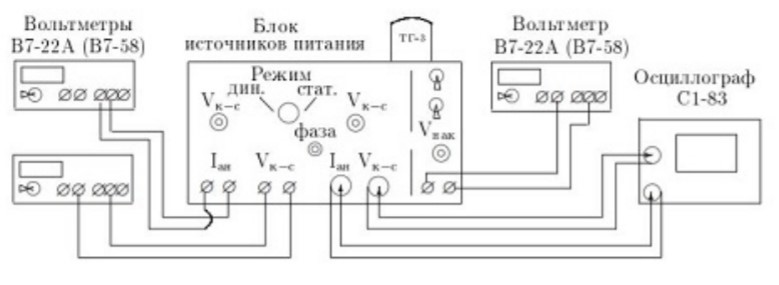
\includegraphics[width = 0.6\textwidth]{3.jpg}
			\caption{Блок-схема экспериментальной установки}
		\end{center}
	\end{figure}
	\section*{Ход работы}
	Снимем с помощью осциллографа ВАХ при двух различных напряжениях, а затем измерим $V_{\max}$, $V_{\min}$ в зависимости от $U_{\text{накала}}$. Все данные, в том числе и изображения, занесем в таблицу.
	\begin{table}[H]
		\centering
		\begin{tabular}{|c|c|c|}
			\hline
			$U_\text{нак}$, В & $U_\text{max}$, В & $U_\text{min}$, В \\ \hline
			3.36   & 4.8    & 9.2    \\ \hline
			3.16   & 5      & 9.4    \\ \hline
		\end{tabular}
	\end{table}
	
\end{document}